\documentclass[border=10pt]{standalone}
\usepackage{tikz}
\usetikzlibrary{arrows.meta,positioning,decorations.pathmorphing,calc}
\usepackage{amsmath,amssymb}

\begin{document}
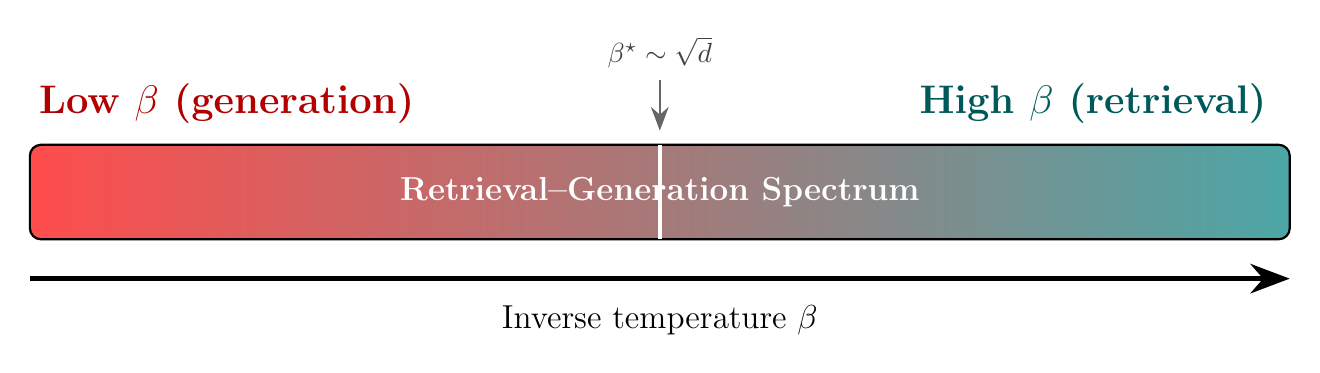
\begin{tikzpicture}

% Main spectrum bar
\def\barlen{16}
\def\barht{1.2}
\def\trans{0.50}   % fraction along bar where beta* sits

% Gradient fill: red (low beta, hot) -> teal (high beta, cold)
\shade[left color=red!70, right color=teal!70, rounded corners=4pt]
    (0,0) rectangle (\barlen,\barht);
\draw[thick, rounded corners=4pt] (0,0) rectangle (\barlen,\barht);

% Beta* marker — bold vertical line
\draw[ultra thick, white] (\barlen*\trans, 0) -- (\barlen*\trans, \barht);

% Scaling law annotation
\node[font=\normalsize, black!75, anchor=south, align=center]
    at (\barlen*\trans, \barht+0.85) {$\beta^{\star} \sim \sqrt{d}$};

% Arrow pointing to marker
\draw[thick, -{Stealth[length=3mm]}, black!60]
    (\barlen*\trans, \barht+0.82) -- (\barlen*\trans, \barht+0.18);

% Beta arrow underneath
\draw[ultra thick, -{Stealth[length=5mm]}] (0,-0.5) -- (\barlen,-0.5);
\node[font=\large, anchor=north] at (\barlen/2, -0.72)
    {Inverse temperature $\beta$};

% Low beta label (left) — red (hot)
\node[font=\Large\bfseries, red!70!black, anchor=south] at (2.5, \barht+0.15)
    {Low $\beta$ (generation)};

% High beta label (right) — teal (cold)
\node[font=\Large\bfseries, teal!70!black, anchor=south]
    at (\barlen-2.5, \barht+0.15) {High $\beta$ (retrieval)};

% Center bar label
\node[font=\large\bfseries, white] at (\barlen/2, \barht/2)
    {Retrieval--Generation Spectrum};

\end{tikzpicture}
\end{document}
